\documentclass[11pt,aspectratio=169]{beamer}

\usepackage[T1]{fontenc}
\usepackage{lmodern}
\usepackage{graphicx}
\usepackage{tikz}
\usetikzlibrary{arrows.meta,positioning,calc,decorations.pathreplacing,overlay-beamer-styles,shapes.geometric,patterns}
\usepackage{pgfplots}
\pgfplotsset{compat=1.17}
\usepackage{amsmath,amssymb,mathtools}
\usepackage{booktabs,tabularx,array,multirow}
\usepackage{appendixnumberbeamer}

\setbeamercovered{transparent=5}
\setbeamertemplate{navigation symbols}{}
\setbeamertemplate{itemize items}[circle]
\setbeamertemplate{itemize subitem}{--}
\setbeamertemplate{footline}[frame number]
\setbeamerfont{framesubtitle}{size=\small}
\setbeamercolor{block title}{fg=black,bg=white!80!black}
\setbeamercolor{block body}{fg=black,bg=white!97!black}
\linespread{1.2}

\newcolumntype{Y}{>{\raggedright\arraybackslash}X}
\newcolumntype{C}{>{\centering\arraybackslash}X}
\newcommand{\1}{\mathbf 1}
\newcommand{\E}{\mathbb E}
\newcommand{\sym}[1]{\ifmmode^{#1}\else\(^{#1}\)\fi}
\definecolor{citecolor}{RGB}{110,110,165}
\definecolor{sourcegray}{RGB}{95,95,95}
\newcommand{\cit}[1]{{\color{citecolor}#1}}
\newcommand{\source}[1]{\par\vspace{0.25em}{\tiny\color{sourcegray}Source: #1}}
\newcommand{\takeaway}[1]{\vfill{\small\textbf{Takeaway.} #1}}

\title{Fertility and Housing Tenure Choice}
\author{Tommaso De Santo}
\date{September 14, 2026}

% The complete pre-refocus source is preserved in archive/september_14_before_slide_refocus_20260910.tex.
% Sequential household exposition; choice-structure comparison and calibration design remain open in CALIBRATION_STATUS.md.
\pdfstringdefDisableCommands{\def\translate#1{#1}}

% Link button pinned to the top-right corner of the frame.
\newcommand{\titlelink}[2]{\makebox[0pt][l]{\begin{tikzpicture}[remember picture,overlay]\node[anchor=north east] at ([xshift=-0.35cm,yshift=-0.32cm]current page.north east) {\hyperlink{#1}{\beamergotobutton{#2}}};\end{tikzpicture}}\ignorespaces}
\begin{document}
{
\setbeamertemplate{footline}{}
\maketitle
}

\begin{frame}{Housing and Fertility}
\begin{center}
\includegraphics[width=0.45\textwidth]{../../Latex/newsweek.png}\hspace{-1em}%
\includegraphics[width=0.45\textwidth]{../../Latex/housingwire.png}\\[-0.8em]
\includegraphics[width=0.45\textwidth]{../../Latex/vox.png}\hspace{-1em}%
\includegraphics[width=0.45\textwidth]{../../Latex/cityjournal.png}
\includegraphics[width=0.8\textwidth]{../../Latex/times.png}
\end{center}
\end{frame}

\begin{frame}[label=intro-channels]{Housing, Fertility, and Tenure Choice}
\textbf{Housing costs affect fertility}, but tenure and wealth matter:
\begin{itemize}
  \item Earlier access to homeownership increases family size \cit{(Fazio et al.\ 2025)}
  \item Credit access raises buying, births, and home size \cit{(Hacamo 2021, Couillard 2025)}
\end{itemize}
\medskip
Children increase how big of a house you need. Key channels:
\begin{itemize}
  \item Owning: tenure segmentation (big houses are often only for sale) \hyperlink{big-units-owned}{\beamergotobutton{Data}}
  \item Wealth: borrowing constraints affect purchase ability
  \item Intergenerational distribution: old people own most of the large dwellings \hyperlink{large-homes-data}{\beamergotobutton{Data}}
\end{itemize}
\vfill
How much can physical space affect fertility?\\
What kind of housing policy is good for natality?
\end{frame}

\begin{frame}{This Paper}
\small
\alert{Question:} how much does access to space shape fertility, and can housing policy change it?

\medskip
\alert{Model:} a lifecycle economy with one housing market, in which children need space
\begin{itemize}\setlength\itemsep{2pt}
  \item Households choose when to try for children; children raise the space they need.
  \item Renting is capped in size: large homes must be bought (tenure segmentation).
  \item Buying requires a down payment: wealth and its timing matter (borrowing constraints).
  \item Households age, save, and bequeath: large homes end up with the old (intergenerational allocation).
\end{itemize}

\medskip
\alert{Quantification:} the U.S. as a transition to a smaller population
\begin{itemize}\setlength\itemsep{2pt}
  \item Calibrate the 2007 economy; fit the 2007--2023 fertility decline with preference shocks.
  \item Treat 2023 as a point on the transition and project forward.
  \item Policy: can a property tax that shifts space to young families raise births?
\end{itemize}
\end{frame}

\section{Model}

\begin{frame}[plain,c,noframenumbering]{}
\centering
{\Large\textbf{Model}}
\end{frame}

\begin{frame}{Environment}
\begin{itemize}
  \item Discrete time, overlapping generations of households
  \item Adult age $a\in[0,J]$ with survival probability $s_a$; working age $a\in[0,a_R]$; fertile window $a\in[a_F^0,a_F^1]$
  \item Children:
  \begin{itemize}
    \item mature stochastically; housing need depends on children at home
    \item are dependents and do not work
  \end{itemize}
  \item Households differ in wealth, housing, family composition, and idiosyncratic labor efficiency $z_t$
  \item Households choose:
  \begin{itemize}
    \item \textbf{Fertility}: whether to attempt the next birth, subject to EV shocks
    \item \textbf{Tenure}: rent or buy, with tenure segmentation, subject to EV shocks
    \item \textbf{Savings}: next-period liquid wealth $b_{t+1}$; mortgages secured by the house
  \end{itemize}
\end{itemize}
\end{frame}

\begin{frame}{Preferences}
\footnotesize
\setlength{\abovedisplayskip}{2pt}\setlength{\belowdisplayskip}{2pt}
$n_t$: children ever born; $m_t$: children currently at home.

\smallskip
\textbf{Flow utility.} CRRA over a consumption aggregator $\mathcal C$ and children at home:
\[
u_t(c_t,s_t;m_t)=\frac{\mathcal C(c_t,s_t;m_t)^{1-\sigma}}{1-\sigma}+\psi_t m_t,\qquad \sigma>0.
\]
\begin{itemize}\setlength\itemsep{1pt}
  \item $\mathcal C_c,\mathcal C_s>0$, concave; children raise consumption and housing needs: $\mathcal C_m<0$.
  \item Children raise the marginal value of space: $\mathcal C_{sm}>0$.
  \item $\psi_t m_t$: direct benefit of children at home; starting a family carries a one-time utility cost $\xi$.
\end{itemize}

\smallskip
\textbf{Housing services.} Households either rent or own; $\chi$ scales owner services:
\[
s_t=\mathbf{1}\{\text{own}\}\,\chi\,h_t+\mathbf{1}\{\text{rent}\}\,h_t^R,\qquad \chi>1.
\]

\smallskip
\textbf{Bequests.} Terminal utility over bequeathable wealth $w^e_{t+1}$ (liquid wealth plus housing value):
\[
B(w_{t+1}^e)=\theta_0\frac{(\theta_1+w_{t+1}^e)^{1-\sigma}}{1-\sigma}.
\]
\end{frame}

\begin{frame}[label=housing-constraints]{Housing, Tenure, and Budget Constraints}
\titlelink{big-units-owned}{Data}
\small
\setlength{\abovedisplayskip}{2pt}\setlength{\belowdisplayskip}{2pt}
\textbf{Income and saving.}
\begin{itemize}\setlength\itemsep{2pt}
  \item After-tax earnings $y_t^d(a,z_t)$ and a lump-sum transfer $T_t$.
  \item One-period bond $b_{t+1}$ at gross rate $R_b$; owners borrow only against the house.
\end{itemize}

\medskip
\textbf{Owning.} Buy $h_t\in[0,\bar h]$ at price $P_t$, arriving with $h_{t-1}$.
\begin{itemize}\setlength\itemsep{2pt}
  \item The house depreciates at rate $\delta_H$ and is taxed at rate $\tau_t^p$.
  \item Selling costs a fraction $\psi^s$ of the sale value.
  \item Buying requires a down payment; the rest is a mortgage secured by the house:
  \[
  b_t+(1-\psi^s)P_t h_{t-1}\geq\mathbf{1}\{h_t\neq h_{t-1}\}(1-\phi)P_t h_t,
  \qquad
  b_{t+1}\geq-\phi P_t h_t.
  \]
\end{itemize}

\medskip
\textbf{Renting.} Rent $h_t^R\in[0,\bar h^R]$ at rent $r_t$ per unit, with $\bar h^R<\bar h$.
\begin{itemize}\setlength\itemsep{2pt}
  \item The largest homes are reachable only through ownership.
\end{itemize}

\end{frame}

\begin{frame}{Fertility and Child Aging}
\small
\begin{itemize}\setlength\itemsep{0.6em}
  \item During fertile ages, households choose each period whether to attempt a birth.
  \item The choice is discrete, with an extreme-value taste shock $\varepsilon_t^F$ of scale $\kappa_1$ for the first birth and $\kappa_C$ for later births.
  \item An attempt succeeds with age-specific probability $\pi_a$ and adds one child.
  \item Children mature stochastically: each dependent child leaves the household with a fixed probability each period, independently of the others.
\end{itemize}
\end{frame}

\begin{frame}{Firms and Earnings}
\small
\begin{itemize}
  \item Competitive firms produce with effective labor:
  \[
  Y_t=A L_t,\qquad w=A,\qquad L_t=\int_{a<a_R} e_a z_t\,dG_t.
  \]
  \item Age- and productivity-dependent earnings:
  \[
  y_t^d(a,z_t)=\begin{cases}
  (1-\tau^{w})\,w e_a z_t,&a<a_R,\\
  \varpi_t,&a\geq a_R.
  \end{cases}
  \]
  \item $e_a$: age--earnings profile; $z_t$: idiosyncratic labor efficiency; $G_t$: distribution of households over states.
  \item Retirees receive a pay-as-you-go pension $\varpi_t$; payroll taxes balance it each period.
\end{itemize}
\end{frame}

\begin{frame}{Housing Supply and Rents}
\small
Housing supply:
\[
H_t^s=H_0\,P_t^{\eta}.
\]
\begin{itemize}
  \item $H_0$: supply scale; $\eta$: supply elasticity.
  \item Rent is the user cost of housing: a competitive landlord who buys at $P_t$, pays depreciation and property tax, and resells at $P_{t+1}$ must earn the bond return,
  \[
  r_t=(R_b+\delta_H+\tau_t^p)P_t-P_{t+1}.
  \]
\end{itemize}
\end{frame}

\begin{frame}[t]{%
\only<1>{The Household's Problem: Housing and Savings}%
\only<2>{The Household's Problem: Fertility Choice}%
}
\vspace{0.3em}
\centering
\scalebox{0.85}{%
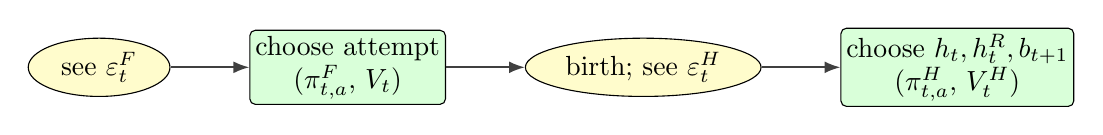
\begin{tikzpicture}[
  node distance=7mm and 10mm, >=Latex,
  see/.style={
    ellipse, draw, fill=yellow!20,
    minimum height=1.3em, minimum width=1.8cm,
    inner sep=2pt, align=center, font=\normalsize
  },
  choose/.style={
    rectangle, draw, fill=green!15, rounded corners=2pt,
    minimum height=1.5em, minimum width=1cm,
    inner sep=2pt, align=center, font=\normalsize
  },
  line/.style={-Latex, semithick, draw=black!75}
]
\node (fertS) [see] {see $\varepsilon_t^F$};
\node (fertD) [choose, right=of fertS, alt=<2>{draw=red, ultra thick}{}] {choose attempt\\($\pi^F_{t,a}$, $V_t$)};
\node (locS)  [see,    right=of fertD] {birth; see $\varepsilon_t^H$};
\node (locD)  [choose, right=of locS,  alt=<1>{draw=red, ultra thick}{}] {choose $h_t,h_t^R,b_{t+1}$\\($\pi^H_{t,a}$, $V^H_t$)};

\draw[line] (fertS) -- (fertD);
\draw[line] (fertD) -- (locS);
\draw[line] (locS)  -- (locD);
\end{tikzpicture}%
}

\par\vspace{0.35em}
\raggedright
\setlength{\abovedisplayskip}{4pt}\setlength{\belowdisplayskip}{4pt}

\only<1>{%
{\footnotesize
\setlength{\abovedisplayskip}{9pt}\setlength{\belowdisplayskip}{9pt}

\textbf{Conditional on the realized family size, choose housing and savings:}
\[
\begin{aligned}
V^H_t(b_t,h_{t-1},z_t,a,n,m)
={}&\E_{\varepsilon_t^H}\max_{h_t,h_t^R,b_{t+1}}
\Bigl\{u_t\big(c_t,\chi h_t+h_t^R;m\big)+\varepsilon_t^H(h_t)\\
&+\beta\E_t\!\left[s_a V_{t+1}(b_{t+1},h_t,z_{t+1},a+1,n_{t+1},m_{t+1})
+(1-s_a)B(w^e_{t+1})\right]\Bigr\}.
\end{aligned}
\]

subject to
\[
c_t+b_{t+1}+r_t h_t^R+(\delta_H+\tau_t^p)P_t h_t
=R_b b_t+y_t^d(a,z_t)+T_t-R_b\mathbf{1}\{h_t\neq h_{t-1}\}P_t\big[h_t-(1-\psi^s)h_{t-1}\big],
\]
\medskip
\[
b_{t+1}\geq-\phi P_t h_t,\qquad
b_t+(1-\psi^s)P_t h_{t-1}\geq\mathbf{1}\{h_t\neq h_{t-1}\}(1-\phi)P_t h_t.
\]
}
}

\only<2>{%
{\footnotesize
\setlength{\abovedisplayskip}{6pt}\setlength{\belowdisplayskip}{6pt}

Waiting and attempting have values
\[
\begin{aligned}
W_t^0&=V^H_t(b_t,h_{t-1},z_t,a,n_t,m_t),\\
W_t^A&=\pi_a\!\left[V^H_t(b_t,h_{t-1},z_t,a,n_t+1,m_t+1)-\xi\1\{n_t=0\}\right]\\
&\quad +(1-\pi_a)V^H_t(b_t,h_{t-1},z_t,a,n_t,m_t).
\end{aligned}
\]
Before fertility tastes, household value is
\[
V_t(b_t,h_{t-1},z_t,a,n_t,m_t)
=\E_{\varepsilon_t^F}\max\{W_t^0+\varepsilon_{t,0}^F,\ W_t^A+\varepsilon_{t,A}^F\}.
\]
Choice probabilities:
\[
\pi^F_{t,a}(b_t,h_{t-1},z_t,n_t,m_t)
=\frac{\exp\{W_t^A/\kappa(n_t)\}}
{\exp\{W_t^A/\kappa(n_t)\}+\exp\{W_t^0/\kappa(n_t)\}},
\]
Here $\kappa(n_t)=\kappa_1$ if $n_t=0$ and $\kappa_C$ otherwise. Expected births equal $\pi_a\pi^F_{t,a}$.
}
}
\end{frame}

\begin{frame}{Equilibrium}
\small
\setlength{\abovedisplayskip}{3pt}\setlength{\belowdisplayskip}{3pt}
Given parameters, an initial population $N_0$, and an initial household distribution $G_0$, an equilibrium is a sequence
\[
\{V_t,\;g_t,\;G_t,\;N_t,\;P_t,\;r_t,\;T_t,\;\varpi_t\}_{t\ge0}
\]
such that, for every $t$:
\begin{enumerate}\setlength\itemsep{3pt}
  \item \textbf{Households.} Given $\{P_s,r_s,T_s,\varpi_s\}_{s\ge t}$, $V_t$ solves the household problem with continuation $V_{t+1}$; the policy functions $g_t$ (fertility, housing, savings) attain it.
  \item \textbf{Markets and government.} Rent is the user cost of housing, the housing market clears, pensions balance payroll taxes, and property-tax revenue is rebated equally.
  \item \textbf{Population.} Births $B_t=\int\pi_a\pi^F_{t,a}\,dG_t$ enter at age zero and persons age with survival $s_a$: $N_{0,t+1}=B_t$, $N_{a+1,t+1}=s_a N_{a,t}$.
  \item \textbf{Consistency.} $G_{t+1}$ follows from $G_t$ under $g_t$ and the idiosyncratic shocks, with entrants making the number of households at each age consistent with $N_{t+1}$.
\end{enumerate}
\end{frame}

\section{Quantification}

\begin{frame}[plain,c,noframenumbering]{}
\centering
{\Large\textbf{Quantification}}
\end{frame}

\begin{frame}[t]{Initial Steady State}
\begin{minipage}[t][0.06\textheight][t]{\textwidth}
\vspace{0pt}
For intuition, summarize housing costs by $p$ and fertility by $n(p;\psi)$.
\end{minipage}\par
\begin{minipage}[t][0.56\textheight][t]{\textwidth}
\vspace{0pt}\centering
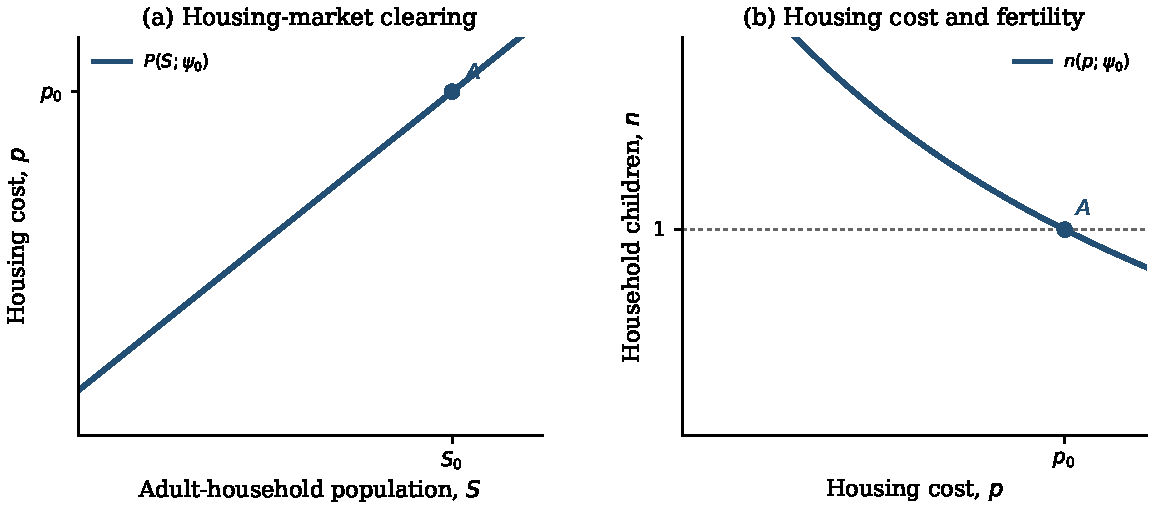
\includegraphics[width=\linewidth,height=0.56\textheight,keepaspectratio]{figures/september_housing_fertility_stage_initial.pdf}
\end{minipage}\par
\begin{minipage}[t][0.16\textheight][t]{\textwidth}
\vspace{0pt}\raggedright\small
At $A$, housing clears at $(S_0,p_0)$ and fertility is at the replacement rate $\bar n$.
\end{minipage}
\end{frame}

\begin{frame}[t,noframenumbering]{Impact}
\begin{minipage}[t][0.06\textheight][t]{\textwidth}
\vspace{0pt}
\mbox{}
\end{minipage}\par
\begin{minipage}[t][0.56\textheight][t]{\textwidth}
\vspace{0pt}\centering
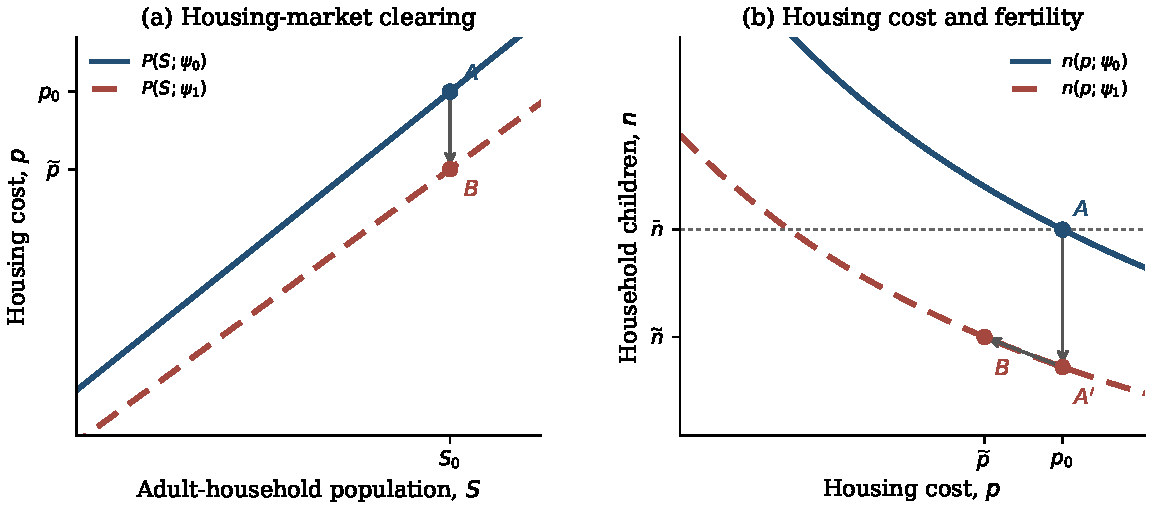
\includegraphics[width=\linewidth,height=0.56\textheight,keepaspectratio]{figures/september_housing_fertility_stage_impact.pdf}
\end{minipage}\par
\begin{minipage}[t][0.16\textheight][t]{\textwidth}
\vspace{0pt}\raggedright\small
A fall from $\psi_0$ to $\psi_1$ lowers fertility at unchanged housing cost: $A\to A'$. Housing costs then adjust at inherited population $S_0$: $A'\to B$.
\end{minipage}
\end{frame}

\begin{frame}[t,noframenumbering]{Demographic Adjustment}
\begin{minipage}[t][0.06\textheight][t]{\textwidth}
\vspace{0pt}
\mbox{}
\end{minipage}\par
\begin{minipage}[t][0.56\textheight][t]{\textwidth}
\vspace{0pt}\centering
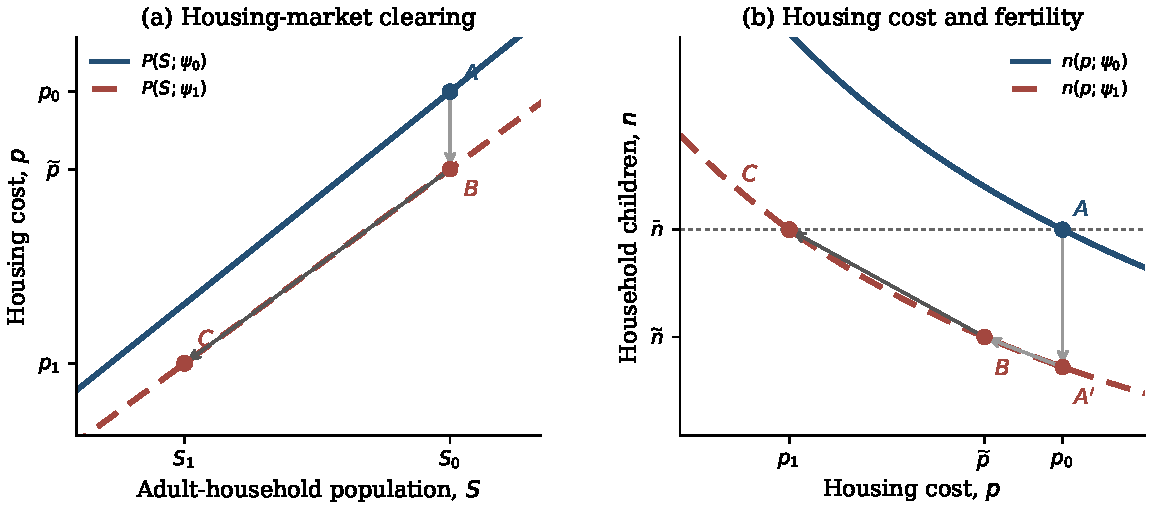
\includegraphics[width=\linewidth,height=0.56\textheight,keepaspectratio]{figures/september_housing_fertility_stage_adjustment.pdf}
\end{minipage}\par
\begin{minipage}[t][0.16\textheight][t]{\textwidth}
\vspace{0pt}\raggedright\small
Smaller entering cohorts reduce housing demand. Lower housing costs partly offset the preference decline; $C$ marks the new stationary outcome.
\end{minipage}
\end{frame}


% Initial tables and fit coordinates: verified_final/selected_target_fit.csv and selected_parameters.csv (2026-09-12).
% Fingerprint c0e266d3a0d430343c469d780d1aedb45fa87f8763c9c938889e0c37daa31de2.

\begin{frame}[t]{Fertility in the United States}
\centering
% Display copies from the verified WDI/CPS series, plotted from 1990; the completed-fertility continuation is rescaled to end at the constant period TFR (top-code filled by author).
\alt<2>{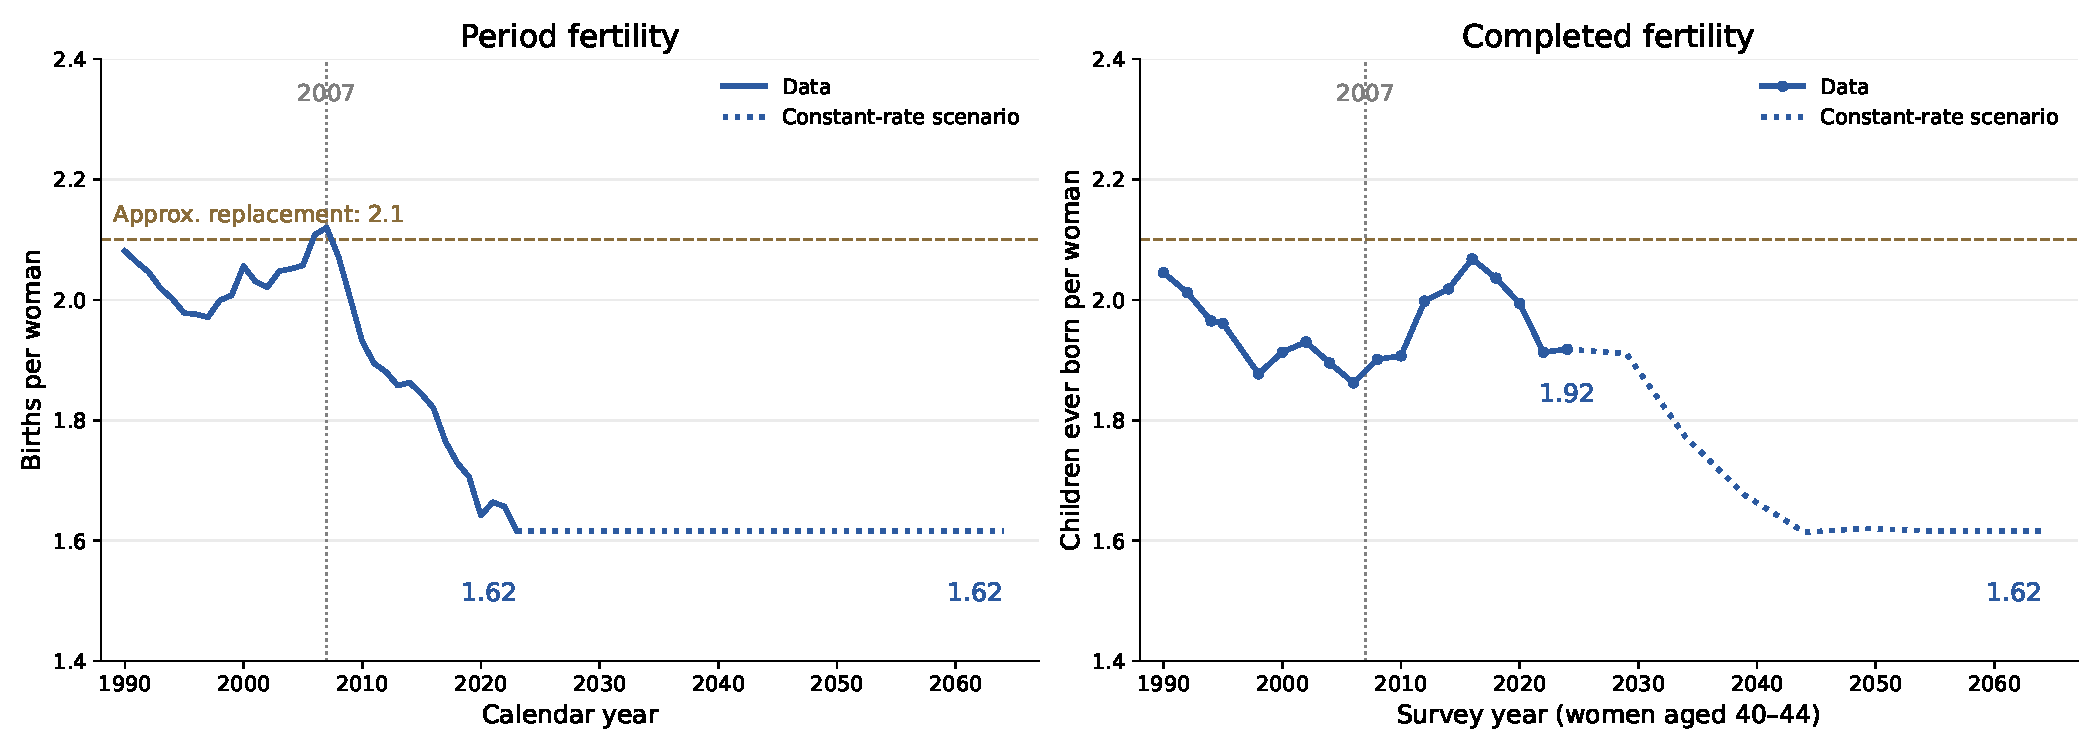
\includegraphics[width=\textwidth,height=0.8\textheight,keepaspectratio]{figures/fertility_introduction_projection_1990.pdf}}{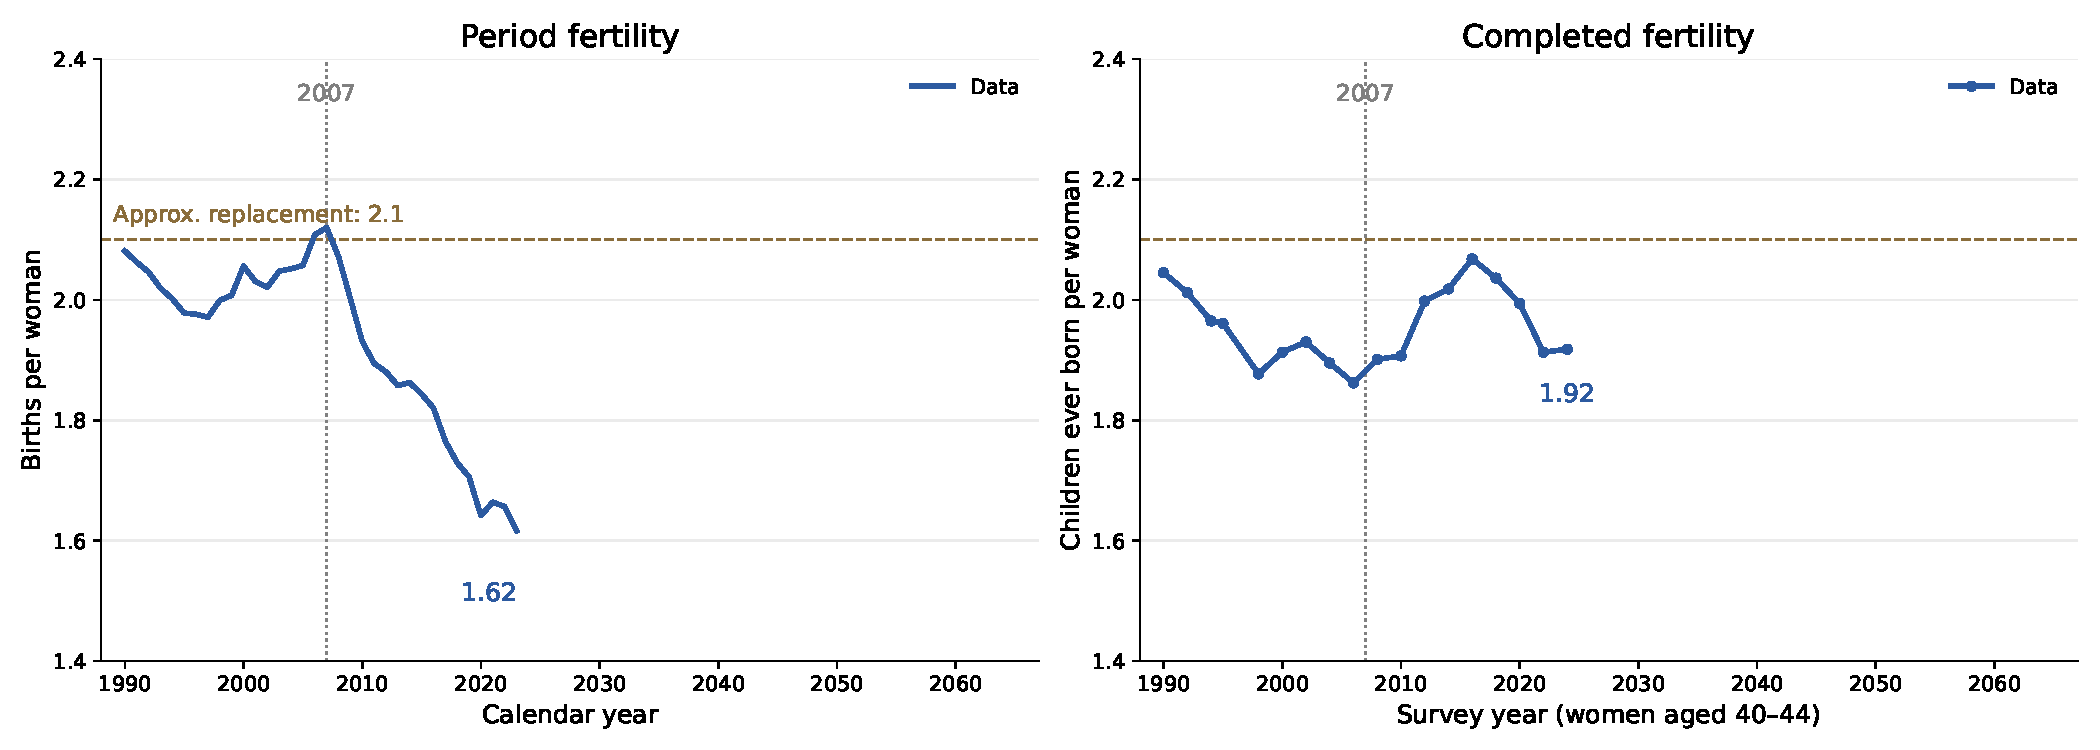
\includegraphics[width=\textwidth,height=0.8\textheight,keepaspectratio]{figures/fertility_introduction_history_1990.pdf}}
\end{frame}

\begin{frame}[label=calibration-overview]{Calibration and Historical Transition}
\titlelink{empirics}{Empirical evidence}
\begin{enumerate}\setlength\itemsep{1.1em}
  \item \textbf{Calibrate the 2007 steady state.}\\
  Match fertility, housing, and wealth moments to determine household parameters.
  \item \textbf{Estimate the sequence of fertility shocks.}\\
  Hold those parameters fixed and match birth rates through 2023 with unanticipated changes in fertility preferences. Carry households and population forward between shocks.
  \item \textbf{Project the economy forward.}\\
  After 2023, hold fertility preferences fixed and solve for prices, housing choices, and population. Compare housing policies from the same 2023 economy.
\end{enumerate}
\medskip
A model period is four calendar years.

\end{frame}

\begin{frame}{Utility Specification}
\small
\[
u_t(c_t,s_t;m_t)=
\frac{\left[\dfrac{c_t^{\alpha_0}\bigl(s_t-\bar h(m_t)\bigr)^{1-\alpha_0}}{e(m_t)}\right]^{1-\sigma}}{1-\sigma}
+\psi_tm_t.
\]
\[
e(m_t)=\left(\frac{2+\omega\, m_t}{2}\right)^{\nu},\qquad
\bar h(m_t)=h_P\mathbf{1}\{m_t>0\}.
\]
\smallskip
Equivalence scale $e(m_t)$ as in Scholz, Seshadri \& Khitatrakun (2006).
\end{frame}


\begin{frame}{Identification}
\footnotesize
Ten parameters are chosen jointly to match twelve moments.

\medskip
\textbf{Fertility}
\vspace{-3pt}\begin{itemize}\setlength\itemsep{0pt}
  \item $\psi_0$, preference for children $\to$ completed fertility
  \item $\xi$, first-birth cost $\to$ childlessness
  \item $\kappa_1$, first-birth taste dispersion $\to$ mean age at first birth, first births after 30
  \item $\kappa_C$, later-birth taste dispersion $\to$ one-child families
\end{itemize}
\vspace{-2pt}
\textbf{Housing}
\vspace{-3pt}\begin{itemize}\setlength\itemsep{0pt}
  \item $h_P$, space requirement of parents $\to$ rooms added at first birth, rooms of 3+ versus 1--2 children
  \item $\chi$, owner premium $\to$ ownership rate
  \item $H_0$, supply scale $\to$ mean rooms
\end{itemize}
\vspace{-2pt}
\textbf{Saving and bequests}
\vspace{-3pt}\begin{itemize}\setlength\itemsep{0pt}
  \item $\beta$, discount factor $\to$ wealth over earnings
  \item $\theta_0$, bequest scale $\to$ bequest flow
  \item $\theta_1$, bequest wealth shift $\to$ old-age p90/median
\end{itemize}
\end{frame}

\begin{frame}{Calibration: Targets and Model}
\footnotesize
\linespread{1}\selectfont
\renewcommand{\arraystretch}{1.12}
\begin{tabularx}{\textwidth}{@{}Xrr@{}}
\toprule
Moment & Target & Model \\
\midrule
Completed fertility & 2.10 & 2.10 \\
Childless, women 40--44 (\%) & 19.8 & 20.7 \\
Exactly one child among mothers, 40--44 (\%) & 21.4 & 20.7 \\
Mean age at first birth (years) & 25.98 & 26.10 \\
First births at age 30+ (\%) & 24.9 & 23.2 \\
\addlinespace[4pt]
Mean occupied rooms (capped at 9) & 5.56 & 6.29 \\
Ownership, heads 30--55 (\%) & 64.8 & 52.4 \\
First-birth room response, $-1$ to $+3$ & 0.720 & 1.011 \\
Rooms: 3+ versus 1--2 resident children & 0.347 & 0.200 \\
\addlinespace[4pt]
Wealth / annual gross earnings & 6.15 & 4.85 \\
Annual bequests / wealth (\%) & 0.88 & 0.86 \\
Wealth/income p90 / median, ages 76--84 & 3.52 & 4.44 \\
\bottomrule
\end{tabularx}\par
\smallskip
\scriptsize Sources: CPS 2004/2006 (children ever born, women 40--44); natality records 2003--2006 (first-birth timing); ACS 2005/2006, 42 metros (rooms, ownership); PSID 2003/2005 (wealth); PSID event study (room response).
\end{frame}
\begin{frame}{Internally Calibrated Parameters}
\footnotesize

\renewcommand{\arraystretch}{1.12}
\begin{tabularx}{\textwidth}{@{}lXr@{}}
\toprule
Parameter & Economic interpretation & Value \\
\midrule
$\beta_{\rm annual}$ & Annual discount factor & 0.990 \\
$\kappa_1$ & First-birth taste dispersion & 0.279 \\
$\kappa_C$ & Later-birth taste dispersion & 0.347 \\
$\chi$ & Owner housing-service multiplier & 1.048 \\
$H_0$ & Housing supply scale & 8.191 \\
$\theta_0$ & Bequest-motive scale & 0.087 \\
$\theta_1$ & Bequest-utility wealth shift & 0.057 \\
$\xi$ & First-birth utility cost & 0.127 \\
$h_P$ & Parenthood space requirement & 2.300 \\
$\psi_0$ & Initial preference for children & 0.160 \\

\bottomrule
\end{tabularx}
\end{frame}

\begin{frame}{Externally Calibrated Parameters}
\footnotesize
\renewcommand{\arraystretch}{1.0}
\begin{tabularx}{\textwidth}{@{}>{\raggedright\arraybackslash}p{0.34\textwidth}>{\raggedright\arraybackslash}p{0.25\textwidth}>{\raggedright\arraybackslash}X@{}}
\toprule
Parameter & Value & Source \\
\midrule
Risk aversion $\sigma$ & 2 & \\
Equivalence scale $(\omega,\nu)$ & $(0.7,\,0.7)$ & Scholz et al.\ (2006) \\
Consumption share $\alpha_0$ & 0.733 & CEX 2019--23, childless renters \\
Housing-supply elasticity $\eta$ & 0.63 & Baum-Snow \& Han (2024) \\
Annual real interest rate $q_{\mathrm{ann}}$ & 2.0\% & Greaney et al.\ (2025) \\
Payroll tax rate $\tau^{w}$ & 17.9\% & OECD U.S. average \\
Financed share $\phi$ & 0.80 & 20\% down payment \\
Depreciation $\delta_H$, property tax $\tau^p$ & 2\%, 1\% per year & \\
Selling cost $\psi^s$ & 6\% & Greaney et al.\ (2025) \\
Rental size cap $\bar h^R$ & 6 rooms & Greaney et al.\ (2025) \\
Ages & 18, 66, 45 & entry, retirement, last fertile age \\
\bottomrule
\end{tabularx}
\end{frame}

\begin{frame}[label=transition-short]{Fertility Transition: 2007--2063}
\titlelink{algo-ss}{Algorithm}
\centering

\includegraphics[width=\textwidth,height=0.84\textheight,keepaspectratio,trim=0 28 0 0,clip]{../output/model/e5f_original_queue_20260913a/terminal_restart_v1/fertility_replay_iter3/output/fertility_fit_2007_2063.pdf}
\end{frame}

\begin{frame}{Full Transition: 2007--2403}
\centering

\includegraphics[width=\textwidth,height=0.84\textheight,keepaspectratio,trim=0 30 0 0,clip]{../output/model/e5f_original_queue_20260913a/terminal_restart_v1/fertility_replay_iter3/output/full_transition_four_panel.pdf}
\end{frame}

\begin{frame}{2023 Data and Model}
\footnotesize
\renewcommand{\arraystretch}{0.90}
\begin{tabularx}{\textwidth}{@{}Xrr@{}}
\toprule
Moment & Data & Model \\
\midrule
Completed fertility, ages 40--44 & 1.92 & 1.70 \\
Childless, ages 40--44 (\%) & 18.8 & 25.0 \\
Exactly one child among mothers, 40--44 (\%) & 22.2 & 25.5 \\
Mean age at first birth (years) & 28.09 & 29.74 \\
First births at age 30+ (\%) & 37.7 & 44.0 \\
\addlinespace[2pt]
Mean occupied rooms (capped at 9) & 5.58 & 6.07 \\
Ownership, heads 30--55 (\%) & 58.7 & 46.9 \\
First-birth room response, $-$1 to +3 & 0.720 & 1.060 \\
Rooms: 3+ versus 1--2 resident children & 0.355 & 0.266 \\
\addlinespace[2pt]
Wealth / annual gross earnings & 6.87 & 5.64 \\
Annual bequests / wealth (\%) & 0.88 & 0.70 \\
Wealth/income p90 / median, ages 76--84 & 3.45 & 3.50 \\
\bottomrule
\end{tabularx}
\end{frame}

\begin{frame}{Lifecycle Fit in 2023}
\centering

\includegraphics[width=\textwidth,height=0.85\textheight,keepaspectratio,trim=0 25 0 0,clip]{../output/model/e5f_original_queue_20260913a/terminal_restart_v1/fertility_replay_iter3/profile_2023/figures/lifecycle_2023.pdf}
\end{frame}

\begin{frame}{Intergenerational Allocation: Model vs Data}
\centering
% Bottom strip clipped to remove the figure's internal status caption.

\includegraphics[width=0.9\linewidth,height=0.5\textheight,keepaspectratio,trim=0 34 0 0,clip]{../output/model/e5f_original_queue_20260913a/terminal_restart_v1/fertility_replay_iter3/profile_2023/figures/intergenerational_allocation_2023.pdf}
\par\centerline{\scriptsize Share of owner-occupied homes with $6+$ rooms; ACS 2023.}
\vspace{4pt}
\raggedright\footnotesize
\begin{itemize}\setlength\itemsep{1pt}
  \item Large homes sit with older households without children; young families hold few.
  \item Coven et al.\ (2025): a rebated property tax moves space from old owners to young households.
  \item Those young households are the ones deciding on children, and children need space.
\end{itemize}
\end{frame}

\begin{frame}{Policy}
\small
\textbf{The experiment of Coven, Golder, Gupta \& Ndiaye (2025)}
\begin{itemize}\setlength\itemsep{2pt}
  \item Tax housing by value; rebate the revenue equally to all households.
  \item Older owners pay more than they get back; young renters get back more than they pay.
  \item House prices fall; constrained young households buy sooner or buy bigger.
\end{itemize}

\medskip
\textbf{This paper}
\begin{itemize}\setlength\itemsep{2pt}
  \item Same experiment: property tax from 1\% to 2\%, equal rebate, from the 2023 economy.
  \item Follow prices, rents, who lives in the large homes, and births along the path.
  \item Does the space that moves to young families turn into children?
\end{itemize}
\end{frame}

\begin{frame}{Policy Results}
\centering
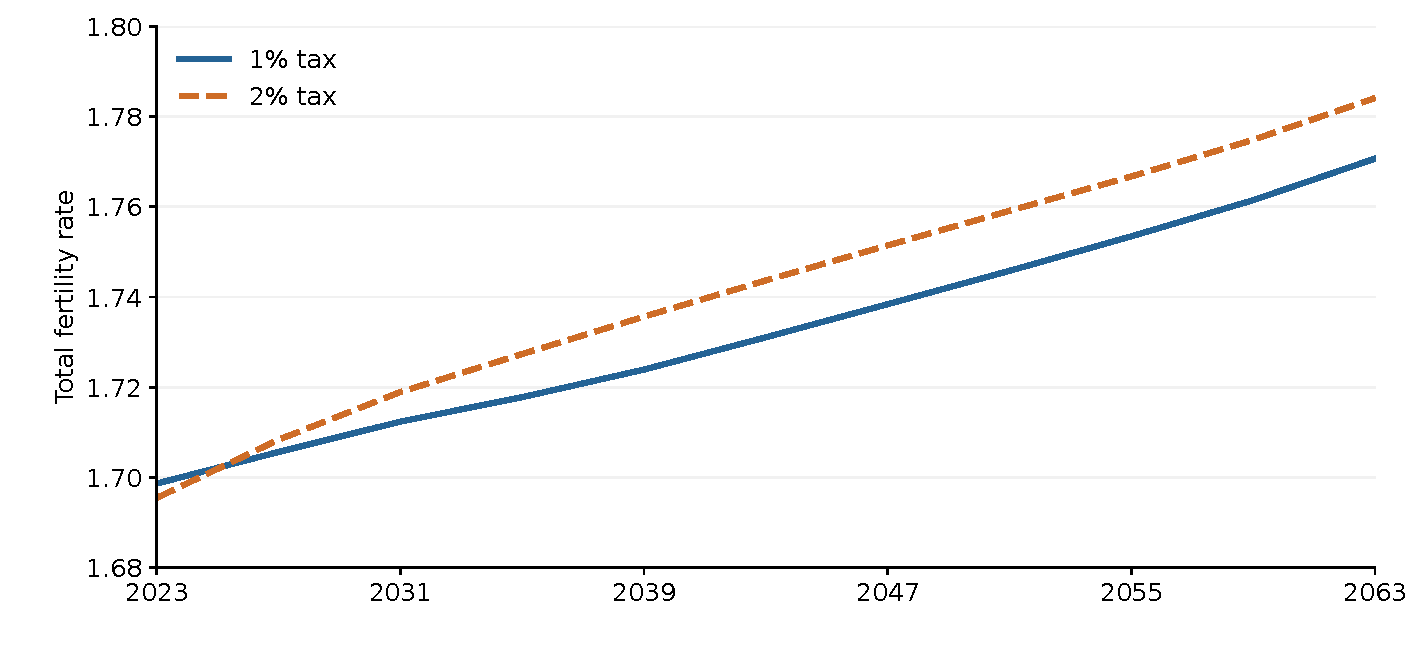
\includegraphics[width=.95\textwidth,height=.70\textheight,keepaspectratio]{../output/model/e5f_original_queue_20260913a/inherited_2023_tax/transition_readout/policy_fertility.pdf}
\end{frame}

\begin{frame}{Conclusion}
\begin{itemize}\setlength\itemsep{1.4em}
  \item A lifecycle model of fertility with realistic housing: tenure, down payments, space
  \item Children need space; large homes must be bought; the old hold most of them
  \item Today is a point on a transition to a smaller population
  \item A rebated property tax can move space toward young families, generating a fertility response
\end{itemize}
\end{frame}

\begin{frame}[plain,c,noframenumbering]{}
\centering{\Huge Thank You!}
\end{frame}

\appendix

\begin{frame}[plain,c,noframenumbering]{}
\centering{\Large\textbf{Appendix}}
\end{frame}



\begin{frame}{The 2023 Equilibrium}
\centering
% Display copy of the price and children panels of patch_readout_fit/figures/equilibrium_2023.pdf, drawn from figure_verification.json.
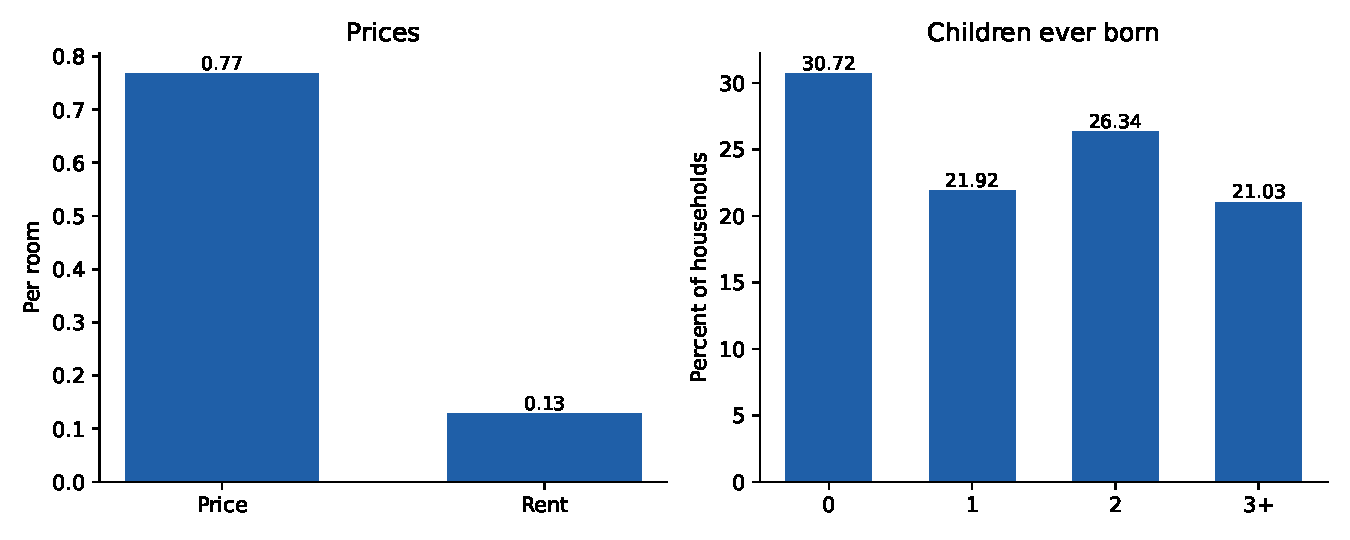
\includegraphics[width=0.9\textwidth,height=0.8\textheight,keepaspectratio]{figures/equilibrium_2023_prices_children.pdf}
\end{frame}

\begin{frame}[label=large-homes-data]{Who Owns the Large Homes}
\titlelink{intro-channels}{Back}
\centering
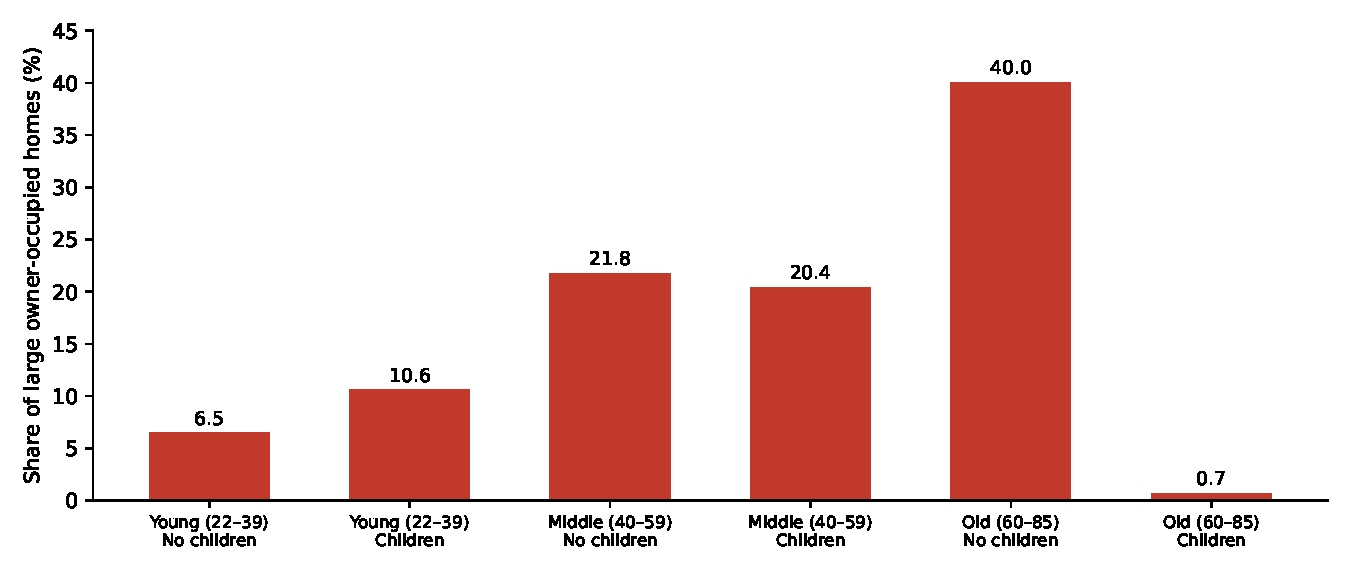
\includegraphics[width=0.9\textwidth,height=0.78\textheight,keepaspectratio]{figures/large_homes_by_age_children_acs2023.pdf}
\par\smallskip
{\scriptsize Owner-occupied homes with $6+$ rooms; ACS 2023.}
\end{frame}

\begin{frame}[label=big-units-owned]{Big Units Are Owned}
\titlelink{housing-constraints}{Back}
\centering
\includegraphics[width=0.77\textwidth,height=0.77\textheight,keepaspectratio]{../code/data/ahs_supply_snapshot/output_ahs_family_unit_menu_national/ahs_tenure_share_within_size.png}
\source{American Housing Survey, 2023.}
\end{frame}

\begin{frame}[label=empirics]{Data}
\titlelink{calibration-overview}{Back}
\begin{itemize}\setlength\itemsep{0.75em}
 \item \textbf{AHS and ACS:} housing sizes, tenure, household composition, and age profiles.
 \item \textbf{PSID:} housing around childbirth, earnings, and wealth by age.
 \item \textbf{CPS and natality records:} completed fertility, childlessness, and birth timing.
 \item \textbf{Census population estimates:} age--sex population and demographic flows.
\end{itemize}

\vfill
Cross-sectional housing patterns discipline access to space; longitudinal data describe housing adjustment around births.
\end{frame}

\begin{frame}{Ownership and Housing Size Around First Birth}
\begin{columns}[T]
\begin{column}{0.48\textwidth}
\centering
{\small Ownership probability}

\smallskip
\includegraphics[width=\linewidth]{../../Outputs/Graphs/own_f_c_y_all.png}
\end{column}
\begin{column}{0.48\textwidth}
\centering
{\small Number of rooms}

\smallskip
\includegraphics[width=\linewidth]{../../Outputs/Graphs/rooms_f_c_y_all.png}
\end{column}
\end{columns}

\medskip
\small Original May event-study coefficients; measurement revisions under review.
\source{PSID; original May event-study estimates.}
\end{frame}

\begin{frame}{Moving Around First Birth}
\begin{columns}[T]
\begin{column}{0.48\textwidth}
\centering
{\small Expansion or better housing}

\smallskip
\includegraphics[width=\linewidth]{../../Outputs/Graphs/mv_s_f_c_y_all.png}
\end{column}
\begin{column}{0.48\textwidth}
\centering
{\small Neighborhood, schools, or proximity}

\smallskip
\includegraphics[width=\linewidth]{../../Outputs/Graphs/mv_n_f_c_y_all.png}
\end{column}
\end{columns}

\medskip
\small Original May event-study coefficients; measurement revisions under review.
\source{PSID; original May event-study estimates.}
\end{frame}

% Closed-population algorithms used by the original household-queue experiment.
% These frames describe the solver and acceptance checks, not convergence results.
\begin{frame}{Steady-State Solution}
Fixed preferences and tax rules; no immigration.

\medskip
\begin{enumerate}\setlength\itemsep{0.55em}
 \item Guess the house price $P$, pension $\varpi$, and rebate $T$; derive rent $r$ from asset pricing.
 \item Solve households backward over age: optimize saving and housing conditional on fertility and tenure, then compute choice probabilities.
 \item Construct the stationary household composition. Set household mass equal to housing supply divided by mean housing per household.
 \item Update $P$, $\varpi$, and $T$ until household entry replaces exits, payroll taxes fund pensions, and property taxes fund equal rebates.
 \item Apply the population law for one period and verify that the distribution and entry queue reproduce themselves; check markets and both budgets.
\end{enumerate}
\end{frame}

\begin{frame}{Transition Solution}
Permanent preference change with a stationary terminal condition.

\medskip
\begin{enumerate}\setlength\itemsep{0.4em}
 \item Fix inherited households and the entry queue; solve the new steady state for the terminal value.
 \item Guess price, pension, and rebate paths $(P_t,\varpi_t,T_t)$; derive rents from asset pricing.
 \item Using these paths, solve households backward in calendar time.
 \item Advance households and entry queues; aggregate housing demand and taxes.
 \item Update all three paths jointly until housing clears and both fiscal budgets balance at every date.
 \item Check terminal distributions and queues against the steady state; extend the horizon to test stability of early responses.
\end{enumerate}
\end{frame}


\end{document}
